\section{26. 根因排序与证据图}

本章先回答一个取证问题：现有本地证据能否支持对应的科学判断。它重要是因为过去多条路线混合了设计承诺、实现状态、训练预算、评价语义和 hosted 结果。本包只采用本地可绑定证据；无法绑定的数字不会被写成性能结论。



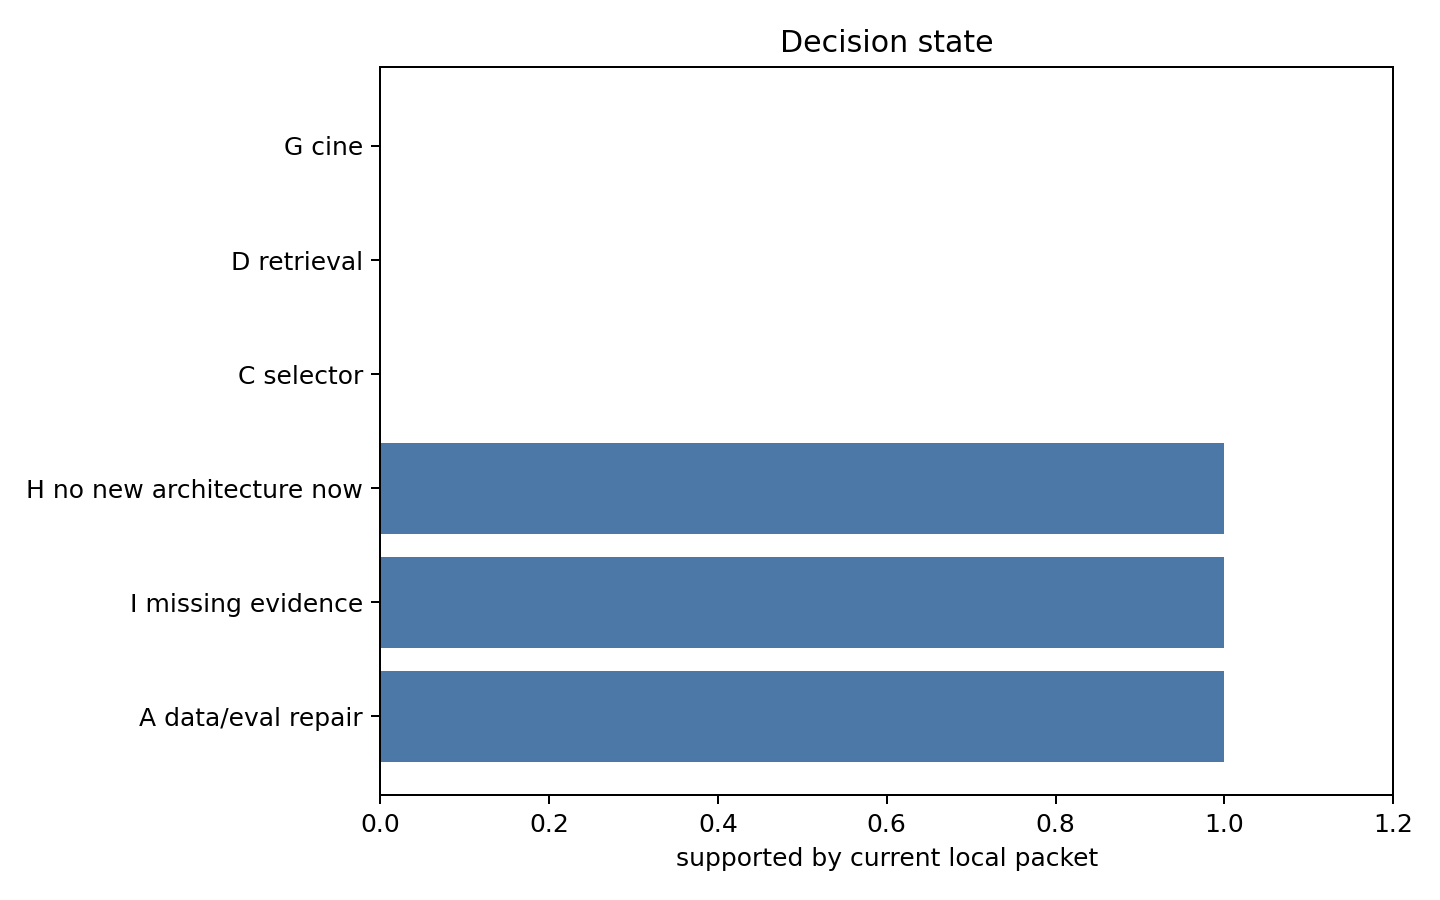
\includegraphics[width=0.92\linewidth]{generated_figures/decision_state.png}

\begin{longtable}{p{0.19\linewidth}p{0.19\linewidth}p{0.19\linewidth}p{0.19\linewidth}p{0.19\linewidth}}
\toprule
root\_cause & evidence & counterevidence & affected\_models & affected\_pathology\\
\midrule
METRIC\_IMPLEMENTATION & remote FP 和 pure-edema/edema-zone 语义已有 known-bad 保护；全量影响未重算。 & not yet fully tested & multiple & scar|pure\_edema|cine\\
CHECKPOINT\_OR\_RECIPE & MoSAIC clean/full-data/hosted recipe 未绑定完成，存在本地证据反转风险。 & not yet fully tested & multiple & scar|pure\_edema|cine\\
DECODER\_CAPABILITY\_LOSS & PRISM decoder-reset 假说合理但 D0-D3 未运行。 & not yet fully tested & multiple & scar|pure\_edema|cine\\
COMPONENT\_NOT\_WIRED & 多个路线需 forward/on-off 才能确认模块是否进入 final logits。 & not yet fully tested & multiple & scar|pure\_edema|cine\\
INSUFFICIENT\_PATHOLOGY\_SIGNAL & feature probe 未运行。 & not yet fully tested & multiple & scar|pure\_edema|cine\\
MULTIMODAL\_MISALIGNMENT & alignment correlation 未运行。 & not yet fully tested & multiple & scar|pure\_edema|cine\\
CINE\_TASK\_DEFINITION & Cine P0/P1 未运行。 & not yet fully tested & multiple & scar|pure\_edema|cine\\
\bottomrule
\end{longtable}



\clearpage